\section{\atk{} learns to translate embeddings without any paired data}
\label{sec:eval_geometry}

% \jm{I am not sure if we want to be describing a new problem in the experiments section. Our sectional flow is already pretty nonstandard. The typical ML paper structure would go Background -> Method -> Experimental Design -> Results. We might want to consider reorganizing things to fit that better}
% \rj{TODO: Need explanation of dataset!}

% In this section, we demonstrate that \atk{} not only translates effectively between each pair of models---\textit{even when baselines fail}---but also produces translations that closely match the geometry of the true embedding vectors of the underlying text, all without access to the original documents.

We first show that \atk{} learns a universal latent space, then demonstrate that this space preserves the geometry of all embeddings.  Therefore, we can use it like a \textbf{universal language of text encoders} to translate their representations without any paired data.

\begin{figure}[t]
    \centering
    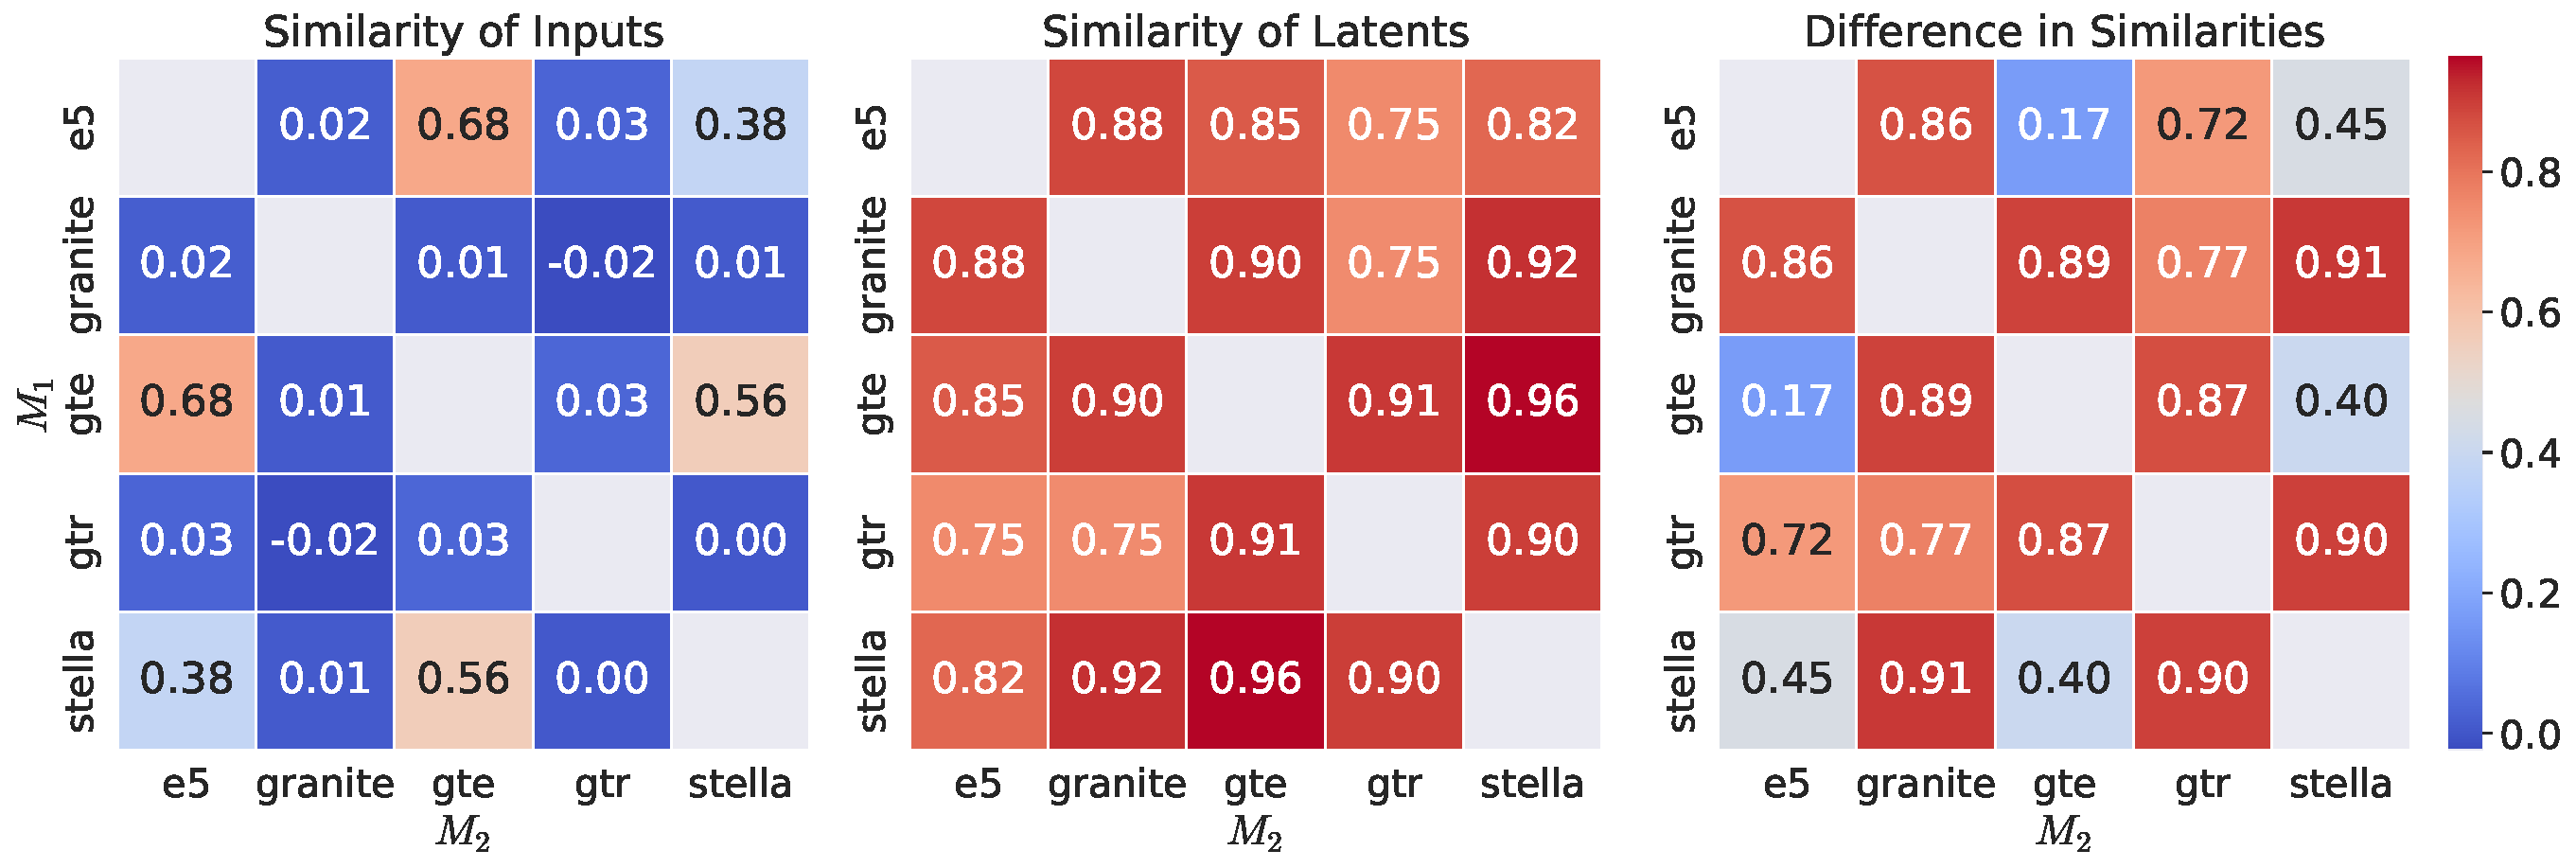
\includegraphics[width=\linewidth]{ims/cosine_heatmaps.pdf}
    \caption{Pairwise cosine similarities of input embeddings (left) and their \atk{} latents (middle) across different embedding pairs. The absolute difference between the heatmaps plots is on the right. All numbers are computed on the same batch of 1024 NQ texts.}
    \label{fig:cosine_heatmaps}
\end{figure}

\shortpara{\atk{} learns a universal latent space.}
\atk{} projects embeddings $M_{1,2,\ldots}$ into a shared latent space via compositions of input adapters ($A_{1,2,\ldots}$) and a shared translator $T$.  \Cref{fig:cosine_heatmaps} shows that even when the embeddings $u_i = M_1(d_i)$ and $v_i = M_2(d_i)$ are far apart (\textit{i.e.,} have low cosine similarity), their representations in \atk{}'s latent space are incredibly close: $T(A_1(u_i)) \approx T(A_2(v_i))$.  \Cref{fig:main} visualizes this (via two-dimensional projections) for \atk{} trained on gte and gtr embeddings: the embeddings are far apart, but their latents 
are \emph{nearly overlapping}.

% As we'll show in the rest of this paper, when passed through output adapters $B_1$ and $B_2$, these nearly-identical latents preserve \textit{geometry and semantics}. So, it follows that the shared latent space must entirely encode the geometric structure of the original embeddings, \textbf{thereby constructing a universal language of text encoders}.

% \vs{To convey the coolness, emphasize that it is not obvious that such a shared latent representation exists and even if it exists, it is not a priori obvious it is possible to discover.}

% \vs{You can also \textbf{start} with baselines, which helps emphasize that naive approaches fail.}


\begin{table}[!b]
    \scriptsize
    \centering
    \begin{tabular}{llrrrrrrrr}
    % \begin{tabular}{ll>{\columncolor{blue!10}}r>{\columncolor{blue!10}}r>{\columncolor{blue!10}}rrrrrrr}
        \toprule
        \multicolumn{2}{c}{} & \multicolumn{3}{c}{\atk{}} & \multicolumn{3}{c}{Naïve Baseline} & \multicolumn{2}{c}{OA Baseline}\\
        \cmidrule(lr){3-5} \cmidrule(lr){6-8}  \cmidrule(lr){9-10} 
        $M_1$ & $M_2$ & $\cos(\cdot)$ $\uparrow$ & Top-1 $\uparrow$ & Rank $\downarrow$ & $\cos(\cdot)$ $\uparrow$ & Top-1 $\uparrow$ & Rank $\downarrow$ & Top-1 $\uparrow$ & Rank $\downarrow$\\
        \midrule
        \multirow{4}{*}{gran.} & gtr & \textbf{0.80 {\tiny (0.0)}} & \textbf{0.99} & \textbf{1.19 {\tiny (0.1)}} & -0.03 {\tiny (0.0)} & 0.00 & 4168.73 {\tiny (9.2)} & 0.00 & 4096.75 {\tiny (9.2)} \\
         & gte & \textbf{0.87 {\tiny (0.0)}} & \textbf{0.95} & \textbf{1.18 {\tiny (0.0)}} & 0.01 {\tiny (0.0)} & 0.00 & 4088.58 {\tiny (9.2)} & 0.00 & 4069.91 {\tiny (9.2)} \\
         & stel. & \textbf{0.79 {\tiny (0.0)}} & \textbf{0.98} & \textbf{1.05 {\tiny (0.0)}} & 0.01 {\tiny (0.0)} & 0.00 & 4208.26 {\tiny (9.2)} & 0.00 & 4096.75 {\tiny (9.2)} \\
         & e5 & \textbf{0.85 {\tiny (0.0)}} & \textbf{0.98} & \textbf{1.11 {\tiny (0.0)}} & 0.02 {\tiny (0.0)} & 0.00 & 4111.60 {\tiny (9.2)} & 0.00 & 4096.75 {\tiny (9.2)} \\
        \midrule
        \multirow{4}{*}{gtr} & gran. & \textbf{0.81 {\tiny (0.0)}} & \textbf{0.99} & \textbf{1.02 {\tiny (0.0)}} & -0.03 {\tiny (0.0)} & 0.00 & 4169.76 {\tiny (9.2)} & 0.00 & 4096.66 {\tiny (9.2)} \\
         & gte & \textbf{0.87 {\tiny (0.0)}} & \textbf{0.93} & \textbf{2.31 {\tiny (0.1)}} & 0.04 {\tiny (0.0)} & 0.00 & 4080.92 {\tiny (9.2)} & 0.00 & 4079.92 {\tiny (9.2)} \\
         & stel. & \textbf{0.80 {\tiny (0.0)}} & \textbf{0.99} & \textbf{1.03 {\tiny (0.0)}} & 0.00 {\tiny (0.0)} & 0.00 & 4198.78 {\tiny (9.2)} & 0.00 & 4096.69 {\tiny (9.2)} \\
         & e5 & \textbf{0.83 {\tiny (0.0)}} & \textbf{0.84} & \textbf{2.88 {\tiny (0.2)}} & 0.03 {\tiny (0.0)} & 0.00 & 4082.84 {\tiny (9.2)} & 0.00 & 4066.42 {\tiny (9.2)} \\
        \midrule
        \multirow{4}{*}{gte} & gran. & \textbf{0.75 {\tiny (0.0)}} & \textbf{0.95} & \textbf{1.22 {\tiny (0.0)}} & 0.01 {\tiny (0.0)} & 0.00 & 4079.81 {\tiny (9.3)} & 0.00 & 4069.23 {\tiny (9.2)} \\
         & gtr & \textbf{0.75 {\tiny (0.0)}} & \textbf{0.91} & \textbf{2.64 {\tiny (0.1)}} & 0.04 {\tiny (0.0)} & 0.00 & 4084.15 {\tiny (9.2)} & 0.00 & 4078.45 {\tiny (9.2)} \\
         & stel. & \textbf{0.89 {\tiny (0.0)}} & \textbf{1.00} & \textbf{1.00 {\tiny (0.0)}} & 0.56 {\tiny (0.0)} & \textbf{1.00} &\textbf{ 1.00 {\tiny (0.0)}} & \textbf{1.00} & \textbf{1.00 {\tiny (0.0)}} \\
         & e5 & \textbf{0.87 {\tiny (0.0)}} & 0.99 & 5.19 {\tiny (0.5)} & 0.68 {\tiny (0.0)} & \textbf{1.00} &\textbf{ 1.00 {\tiny (0.0)}} & \textbf{1.00} & \textbf{1.00 {\tiny (0.0)}} \\
        \midrule
        \multirow{4}{*}{stel.} & gran. & \textbf{0.80 {\tiny (0.0)}} & \textbf{0.98} & \textbf{1.08 {\tiny (0.0)}} & 0.01 {\tiny (0.0)} & 0.00 & 4209.08 {\tiny (9.3)} & 0.00 & 4096.88 {\tiny (9.2)} \\
         & gtr & \textbf{0.82 {\tiny (0.0)}} & \textbf{1.00} & \textbf{1.10 {\tiny (0.0)}} & 0.00 {\tiny (0.0)} & 0.00 & 4192.31 {\tiny (9.2)} & 0.00 & 4096.63 {\tiny (9.2)} \\
         & gte & \textbf{0.92 {\tiny (0.0)}} & \textbf{1.00} & \textbf{1.00 {\tiny (0.0)}} & 0.56 {\tiny (0.0)} & \textbf{1.00} & \textbf{1.00 {\tiny (0.0)}} & \textbf{1.00} & \textbf{1.00 {\tiny (0.0)}} \\
         & e5 & \textbf{0.86 {\tiny (0.0)}} & \textbf{1.00} & \textbf{1.00 {\tiny (0.0)}} & 0.38 {\tiny (0.0)} & 0.99 & 1.03 {\tiny (0.0)} & \textbf{1.00} & \textbf{1.00 {\tiny (0.0)}} \\
        \midrule
        \multirow{4}{*}{e5} & gran. & \textbf{0.81 {\tiny (0.0)}} & \textbf{0.99} & \textbf{2.20 {\tiny (0.2)}} & 0.02 {\tiny (0.0)} & 0.00 & 4120.60 {\tiny (9.3)} & 0.00 & 4096.36 {\tiny (9.2)} \\
         & gtr & \textbf{0.74 {\tiny (0.0)}} & \textbf{0.82} & \textbf{2.56 {\tiny (0.0)}} & 0.03 {\tiny (0.0)} & 0.00 & 4080.76 {\tiny (9.3)} & 0.00 & 4065.74 {\tiny (9.2)} \\
         & gte & \textbf{0.90 {\tiny (0.0)}} & \textbf{1.00} & 1.01 {\tiny (0.0)} & 0.68 {\tiny (0.0)} & \textbf{1.00} & \textbf{1.00 {\tiny (0.0)}} & \textbf{1.00} & \textbf{1.00 {\tiny (0.0)}} \\
         & stel. & \textbf{0.78 {\tiny (0.0)}} & \textbf{1.00} & \textbf{1.00 {\tiny (0.0)}} & 0.38 {\tiny (0.0)} & \textbf{1.00} & \textbf{1.00 {\tiny (0.0)}} & \textbf{1.00} & \textbf{1.00 {\tiny (0.0)}} \\
        \bottomrule\\[-1.6ex]
    \end{tabular}
    \caption{In-distribution translations: \atk{}s trained on NQ and evaluated on a 65536 text subset of NQ (chunked in batches of size 8192). The rank metric varies from 1 to 8192, thus 4096 corresponds to a random ordering. Since Optimal Assignment is a matching method, cosine distances are not applicable.  Standard errors are shown in parentheses. Bold denotes best value.}
    \label{tab:embedding_comparison}
\end{table}

\shortpara{\atk{} translations mirror target geometry.}
\Cref{tab:embedding_comparison} shows that \atk{} generates embeddings with near-optimal assignment across model pairs, achieving cosine similarity scores up to 0.92, top-1 accuracies up to 100\%, and ranks as low as 1. In same-backbone pairings (e.g., (gte, e5)), \atk{}'s top-1 accuracy and rank are comparable to both the naïve baseline and (surprisingly) the oracle-aided optimal assignment. Although the embeddings generated by \atk{} are significantly closer to the ground truth than the naïve baseline, in same-backbone pairings the embeddings are close enough to be compatible.  In cross-backbone pairings, \atk{} is far superior on all metrics, while baseline methods perform similarly to random guessing.

% In particular, given that the evaluation set is chunked in batches of size $8192$ (for computational efficiency), the baseline methods' performance is no better than random in cross-backbone scenarios. This suggests that conventional matching approaches fail to capture structural relationships between embedding spaces unless initial cosine similarities are already sufficiently high.

% \vs{You train on a million embeddings but measure on 8000.  A few words would be helpful + mention that your test set is disjoint from training (is it?)}


\begin{table}[t]
    \scriptsize
    \centering
    \begin{tabular}{llrrr|rrr}
        \toprule
        \multicolumn{2}{c}{} & \multicolumn{3}{c}{TweetTopic} & \multicolumn{3}{c}{MIMIC}\\
        \cmidrule(lr){3-5} \cmidrule(lr){6-8}
        $M_1$ & $M_2$ & $\cos(\cdot)$ $\uparrow$& Top-1 $\uparrow$& Rank $\downarrow$& $\cos(\cdot)$ $\uparrow$& Top-1 $\uparrow$& Rank $\downarrow$\\
        \midrule
        \multirow{4}{*}{gran.} & gtr & 0.74 {\tiny (0.0)} & 0.99 & 1.09 {\tiny (0.1)} & 0.74 {\tiny (0.0)} & 0.60 & 23.38 {\tiny (1.6)} \\
        & gte & 0.85 {\tiny (0.0)} & 0.95 & 1.26 {\tiny (0.1)} & 0.85 {\tiny (0.0)} & 0.08 & 346.21 {\tiny (7.8)} \\
        & stel. & 0.77 {\tiny (0.0)} & 0.96 & 1.11 {\tiny (0.0)} & 0.72 {\tiny (0.0)} & 0.13 & 242.23 {\tiny (6.1)} \\
        & e5 & 0.83 {\tiny (0.0)} & 0.87 & 3.10 {\tiny (0.7)} & 0.84 {\tiny (0.0)} & 0.12 & 361.06 {\tiny (8.7)} \\
        \midrule
        \multirow{4}{*}{gtr} & gran. & 0.79 {\tiny (0.0)} & 0.98 & 2.41 {\tiny (0.6)} & 0.78 {\tiny (0.0)} & 0.51 & 35.27 {\tiny (1.9)} \\
        & gte & 0.85 {\tiny (0.0)} & 0.96 & 1.29 {\tiny (0.2)} & 0.84 {\tiny (0.0)} & 0.12 & 279.56 {\tiny (6.9)} \\
        & stel. & 0.77 {\tiny (0.0)} & 0.96 & 1.10 {\tiny (0.0)} & 0.72 {\tiny (0.0)} & 0.27 & 127.92 {\tiny (4.4)} \\
        & e5 & 0.80 {\tiny (0.0)} & 0.53 & 13.38 {\tiny (1.2)} & 0.82 {\tiny (0.0)} & 0.01 & 1413.80 {\tiny (18.3)} \\
        \midrule
        \multirow{4}{*}{gte} & gran. & 0.73 {\tiny (0.0)} & 0.94 & 1.33 {\tiny (0.1)} & 0.73 {\tiny (0.0)} & 0.09 & 342.15 {\tiny (7.8)} \\
        & gtr & 0.71 {\tiny (0.0)} & 0.95 & 1.29 {\tiny (0.1)} & 0.69 {\tiny (0.0)} & 0.12 & 256.63 {\tiny (6.4)} \\
        & stel. & 0.86 {\tiny (0.0)} & 1.00 & 1.00 {\tiny (0.0)} & 0.85 {\tiny (0.0)} & 1.00 & 1.00 {\tiny (0.0)} \\
        & e5 & 0.83 {\tiny (0.0)} & 0.91 & 1.57 {\tiny (0.2)} & 0.86 {\tiny (0.0)} & 0.54 & 17.71 {\tiny (0.9)} \\
        \midrule
        \multirow{4}{*}{stel.} & gran. & 0.79 {\tiny (0.0)} & 0.99 & 1.09 {\tiny (0.1)} & 0.77 {\tiny (0.0)} & 0.14 & 221.95 {\tiny (5.9)} \\
        & gtr & 0.77 {\tiny (0.0)} & 1.00 & 1.00 {\tiny (0.0)} & 0.75 {\tiny (0.0)} & 0.56 & 17.70 {\tiny (1.0)} \\
        & gte & 0.90 {\tiny (0.0)} & 1.00 & 1.00 {\tiny (0.0)} & 0.91 {\tiny (0.0)} & 1.00 & 1.00 {\tiny (0.0)} \\
        & e5 & 0.85 {\tiny (0.0)} & 0.98 & 1.05 {\tiny (0.0)} & 0.85 {\tiny (0.0)} & 0.51 & 26.33 {\tiny (1.2)} \\
        \midrule
        \multirow{4}{*}{e5} & gran. & 0.79 {\tiny (0.0)} & 0.98 & 1.08 {\tiny (0.0)} & 0.78 {\tiny (0.0)} & 0.21 & 151.09 {\tiny (4.6)} \\
        & gtr & 0.67 {\tiny (0.0)} & 0.80 & 3.10 {\tiny (0.6)} & 0.66 {\tiny (0.0)} & 0.01 & 1029.64 {\tiny (14.9)} \\
        & gte & 0.87 {\tiny (0.0)} & 0.99 & 1.02 {\tiny (0.0)} & 0.87 {\tiny (0.0)} & 0.60 & 32.59 {\tiny (2.6)} \\
        & stel. & 0.75 {\tiny (0.0)} & 0.98 & 1.06 {\tiny (0.0)} & 0.75 {\tiny (0.0)} & 0.46 & 32.12 {\tiny (1.4)} \\
        \bottomrule\\[-1.6ex]
    \end{tabular}
    \caption{Out-of-distribution translations: \atk{}s trained on NQ and evaluated on the entire TweetTopic test set (800 tweets) and an 8192-record subset of MIMIC. The rank metric varies from 1 to 800 (for TweetTopic) and 8192 (for MIMIC), thus 400 and, respectively, 4096 correspond to a random ordering. Standard errors are shown in parentheses.}
    \label{tab:embeddings_ood}
\end{table}

\Cref{tab:embeddings_ood} shows that this performance extends to out-of-distribution data.  Our \atk{} translators were trained on NQ (drawn from Wikipedia), yet exhibit high cosine similarity, high accuracy, and low rank when evaluated on tweets (which are far more colloquial and use emojis) and medical records (which contain domain-specific jargon unlikely to appear in NQ). In \Cref{sec:full_ood}, we show that baseline methods fail on cross-backbone embedding pairs.


\begin{table}[!b]
    \scriptsize
    \centering
    \begin{tabular}{llrrrrr}
        \toprule
        \multicolumn{2}{c}{} & \multicolumn{3}{c}{\atk{}} & \multicolumn{2}{c}{OA Baseline}\\
        \cmidrule(lr){3-5} \cmidrule(lr){6-7}
        $M_1$ & $M_2$ & $\cos(\cdot)$ $\uparrow$& Top-1 $\uparrow$& Rank $\downarrow$& Top-1 $\uparrow$& Rank $\downarrow$\\
        \midrule
        gran. & \multirow{5}{*}{clip} & \textbf{0.78 {\tiny (0.0)}} & \textbf{0.35} & \textbf{226.62} {\tiny (3.2)} & 0.00 & 4096.32 {\tiny (9.2)}\\
        gtr & & \textbf{0.73 {\tiny (0.0)}} & \textbf{0.13} & \textbf{711.23} {\tiny (5.9)} & 0.00 & 4096.71 {\tiny (9.2)} \\
        gte & & \textbf{0.62 {\tiny (0.0)}} & \textbf{0.00} & \textbf{3233.41} {\tiny (9.8)} & 0.00 & 4096.32 {\tiny (9.2)}\\
        stel. & & \textbf{0.77 {\tiny (0.0)}} & \textbf{0.31} & \textbf{286.69} {\tiny (3.6)} & 0.00 & 4096.60 {\tiny (9.2)} \\
        e5 & & \textbf{0.64 {\tiny (0.0)}} & \textbf{0.01} & \textbf{2568.21} {\tiny (9.4)} & 0.00 & 4096.78 {\tiny (9.2)}\\
        \midrule
        \multirow{5}{*}{clip} & gran. & \textbf{0.74 {\tiny (0.0)}} & \textbf{0.72} & \textbf{4.46} {\tiny (0.1)} & 0.00 & 4096.36 {\tiny (9.2)} \\
         & gtr & \textbf{0.67 {\tiny (0.0)}} & \textbf{0.27} & \textbf{155.11} {\tiny (2.1)} & 0.00 & 4096.80 {\tiny (9.2)} \\
         & gte & \textbf{0.75 {\tiny (0.0)}} & \textbf{0.00} & \textbf{2678.90} {\tiny (8.9)} & 0.00 & 4096.12 {\tiny (9.2)} \\
         & stel. & \textbf{0.72 {\tiny (0.0)}} & \textbf{0.61} & \textbf{22.50} {\tiny (0.5)} & 0.00 & 4096.47 {\tiny (9.2)} \\
         & e5 & \textbf{0.73 {\tiny (0.0)}} & \textbf{0.01} & \textbf{1692.28} {\tiny (8.2)} & 0.00 & 4096.44 {\tiny (9.2)} \\
        \bottomrule\\[-1.6ex]
    \end{tabular}
    \caption{Translations between unimodal and multimodal (CLIP) embeddings: \atk{}s trained on NQ and evaluated on a 65536 text subset of NQ (chunked in batches of size 8192). Rank varies from 1 to 8192, thus 4096 corresponds to a random ordering. Since the embedding dimensionalities are different, the naive baseline does not apply. Bold denotes best value.}
    \label{tab:CLIP_nq}
\end{table} 

Finally, \Cref{tab:CLIP_nq} shows that \atk{} can even translate to and from the space of CLIP, a multimodal embedding model which was trained in part on \emph{image} data.  While the translations are not as strong as in \Cref{tab:embedding_comparison}, \atk{} consistently outperforms the optimal assignment baseline. These results show that promise of our method at adapting to new modalities: in particular, the embedding space of CLIP has been successfully connected to other modalities such as heatmaps, audio, and depth charts \citep{girdhar2023imagebind}.

% Stronger methods and/or better hyperparameters may yield even better translations.  Alternatively, it may be possible to translate to and from CLIP using granite or stella as intermediate representations. We leave this to future work.



% \begin{figure}[h]
%     \centering
%     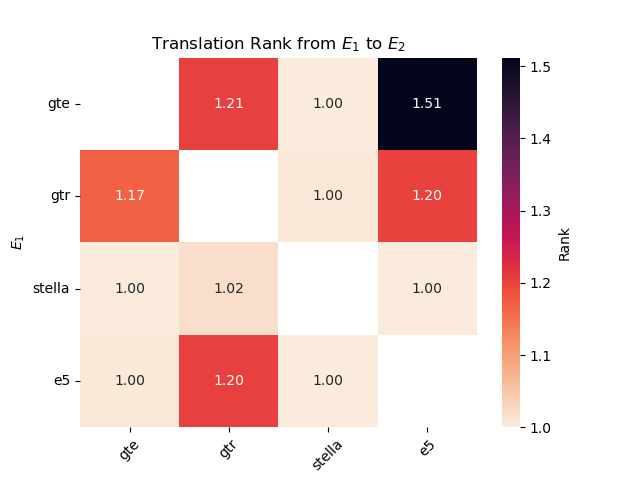
\includegraphics[width=0.6\linewidth]{ims/heatmap_nq.png}
%     \caption{NQ Rank}
%     \label{fig:nq}
% \end{figure}


%%%%%%%%%%%%%%%%%%%% SECTION BREAK %%%%%%%%%%%%%%%%%%%%

\section{Using \atk{} translations to extract information}
\label{sec:eval_semantics}

In this section, we show that \atk{} translations not only preserve the geometric structure of embeddings but also retain sufficient semantics to enable attribute inference.

% In \Cref{sec:eval_geometry} we demonstrated that \atk{} translations faithfully preserve geometric structure. In this section, we extend that result to show that they additionally retain the semantics of the original source embeddings: a capability that has important security implications. 

%Vector databases underpin modern search by indexing data as embeddings. In a breach of such a system where the encoder and any input–embedding pairs are unknown, we show that attackers can \textit{still} extract sensitive information from raw vectors \textit{with no other knowledge}.


\begin{table}[!t]
    \scriptsize
    \centering
    \begin{tabular}{llcccc|cccc}
        \toprule
        \multicolumn{2}{c}{} & \multicolumn{4}{c}{TweetTopic ($k=1$)} & \multicolumn{4}{c}{MIMIC ($k=10$)}\\
        \cmidrule(lr){3-6} \cmidrule(lr){7-10}
        $M_1$ & $M_2$ & \atk{} & Naïve & $M_1$ & $M_2$ & \atk{} & Naïve & $M_1$ & $M_2$ \\
        \midrule
        \multirow{4}{*}{gran.} & gtr & 0.25 & 0.10 & 0.30 & 0.24 & 0.19 & 0.11 & 0.76 & 0.88 \\
        & gte & 0.32 & 0.09 & 0.30 & 0.34 & 0.36 & 0.13 & 0.76 & 1.00 \\
        & stel. & 0.24 & 0.10 & 0.30 & 0.28 & 0.27 & 0.04 & 0.76 & 0.96 \\
        & e5 & 0.31 & 0.18 & 0.30 & 0.31 & 0.19 & 0.20 & 0.76 & 0.97 \\
        \midrule
        \multirow{4}{*}{gtr} & gran. & 0.34 & 0.08 & 0.24 & 0.30 & 0.16 & 0.12 & 0.88 & 0.76 \\
        & gte & 0.33 & 0.13 & 0.24 & 0.34 & 0.28 & 0.05 & 0.88 & 1.00 \\
        & stel. & 0.30 & 0.10 & 0.24 & 0.28 & 0.25 & 0.07 & 0.88 & 0.96 \\
        & e5 & 0.30 & 0.04 & 0.24 & 0.31 & 0.09 & 0.09 & 0.88 & 0.97 \\
        \midrule
        \multirow{4}{*}{gte} & gran. & 0.37 & 0.04 & 0.34 & 0.30 & 0.18 & 0.11 & 1.00 & 0.76 \\
        & gtr & 0.24 & 0.13 & 0.34 & 0.24 & 0.10 & 0.03 & 1.00 & 0.88 \\
        & stel. & 0.31 & 0.20 & 0.34 & 0.28 & 0.68 & 0.83 & 1.00 & 0.96 \\
        & e5 & 0.37 & 0.30 & 0.34 & 0.31 & 0.37 & 0.63 & 1.00 & 0.97 \\
        \midrule
        \multirow{4}{*}{stel.} & gran. & 0.35 & 0.07 & 0.28 & 0.30 & 0.23 & 0.09 & 0.96 & 0.76 \\
        & gtr & 0.26 & 0.13 & 0.28 & 0.24 & 0.22 & 0.09 & 0.96 & 0.88 \\
        & gte & 0.38 & 0.36 & 0.28 & 0.34 & 0.90 & 0.98 & 0.96 & 1.00 \\
        & e5 & 0.35 & 0.34 & 0.28 & 0.31 & 0.38 & 0.46 & 0.96 & 0.97 \\
        \midrule
        \multirow{4}{*}{e5} & gran. & 0.33 & 0.15 & 0.31 & 0.30 & 0.14 & 0.07 & 0.97 & 0.76 \\
        & gtr & 0.26 & 0.22 & 0.31 & 0.24 & 0.11 & 0.04 & 0.97 & 0.88 \\
        & gte & 0.34 & 0.28 & 0.31 & 0.34 & 0.47 & 0.66 & 0.97 & 1.00 \\
        & stel. & 0.26 & 0.16 & 0.31 & 0.28 & 0.36 & 0.40 & 0.97 & 0.96 \\
        \bottomrule\\[-1.6ex]
    \end{tabular}
    \caption{Information leakage via top-$k$ zero-shot attribute inference: \atk{}s trained on NQ and evaluated on the TweetTopic test set (800 tweets) and an 8192-record subset of MIMIC. $M_1$ and $M_2$ represent \textit{ideal} zero-shot inference: attributes and embeddings are encoded using the same model.}
    \label{tab:tweet_topic_mimic_class}
\end{table}


\begin{wrapfigure}{r}{0.42\textwidth}
    \centering
    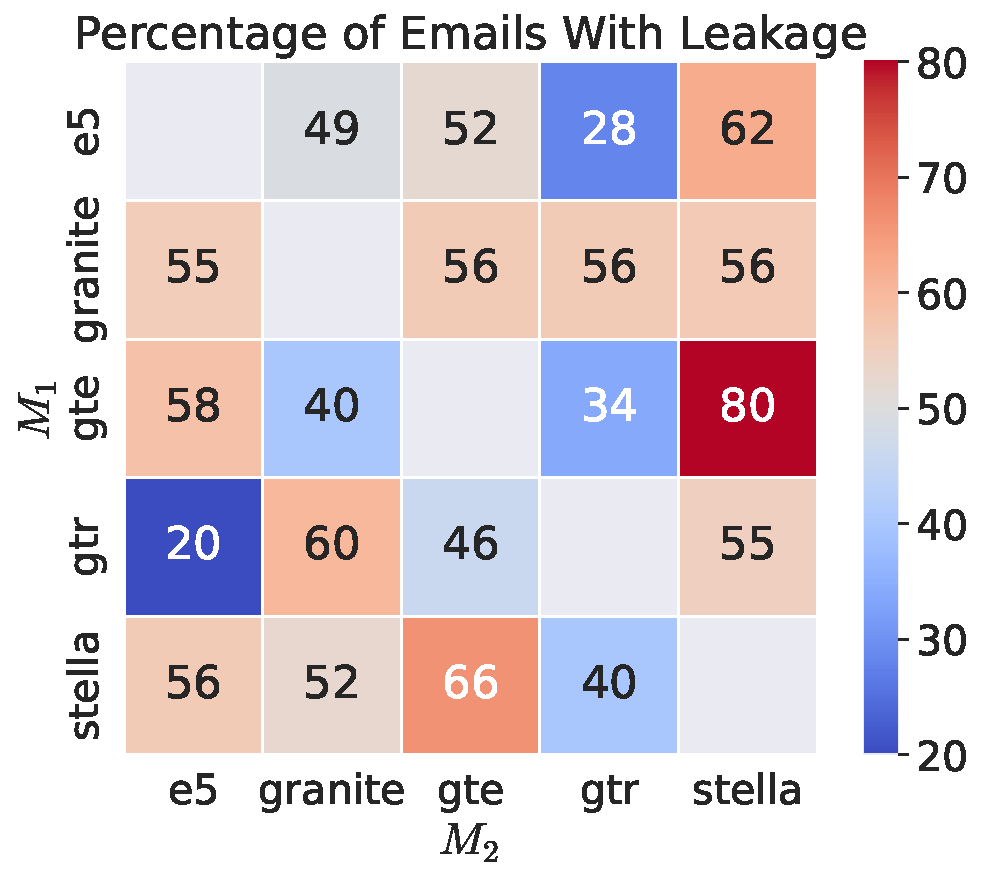
\includegraphics[width=0.37\textwidth]{ims/enron_heatmap.pdf}
      \caption{Leakage of information via inversion. Trained on NQ and evaluated on a 50-email subset of the Enron Email Corpus. Cells denote judge accuracy.}
    \label{fig:enron_heatmap}
\end{wrapfigure}

\shortpara{Zero-shot attribute inference.}
\label{sec:tweet_classification}
\Cref{tab:tweet_topic_mimic_class} shows that attribute inference on \atk{} translations consistently outperforms the naïve baseline and often does better than the ideal zero-shot baseline which performs inference on ground-truth document and attribute embeddings in the same space (this baseline is imaginary since these embeddings are not available in our setting).


% despite translating out-of-distribution tweets, \atk{} preserves sufficient semantic information from the original embedding space to enable effective zero-shot attribute extraction. In fact, attribute extraction from our translated embeddings consistently outperforms the  and frequently surpasses even hypothetical zero-shot extractions performed directly on the untranslated source or target embeddings. We hypothesize that this improved performance arises because the universal latent space captures and integrates shared knowledge from both embedding spaces.


% \paragraph{Case study: extracting disease information from medical records}
\label{sec:mimic_classification}
\atk{} translations even work for embeddings of medical records, which are much further from the training distribution than tweets.  The attributes in this case are MedCAT disease descriptions, very few of which occur in the training data.  Attribute inference on translated embeddings is comparable to the naïve baseline in same-backbone pairings and outperforms it (often greatly) in cross-backbone pairings.  The fact that \atk{} preserves the semantics of concepts like "alveolar periostitis" (which never appears in its training data) is evidence that its latent space is indeed a universal representation.



% \begin{figure}[t]
%     \centering
%     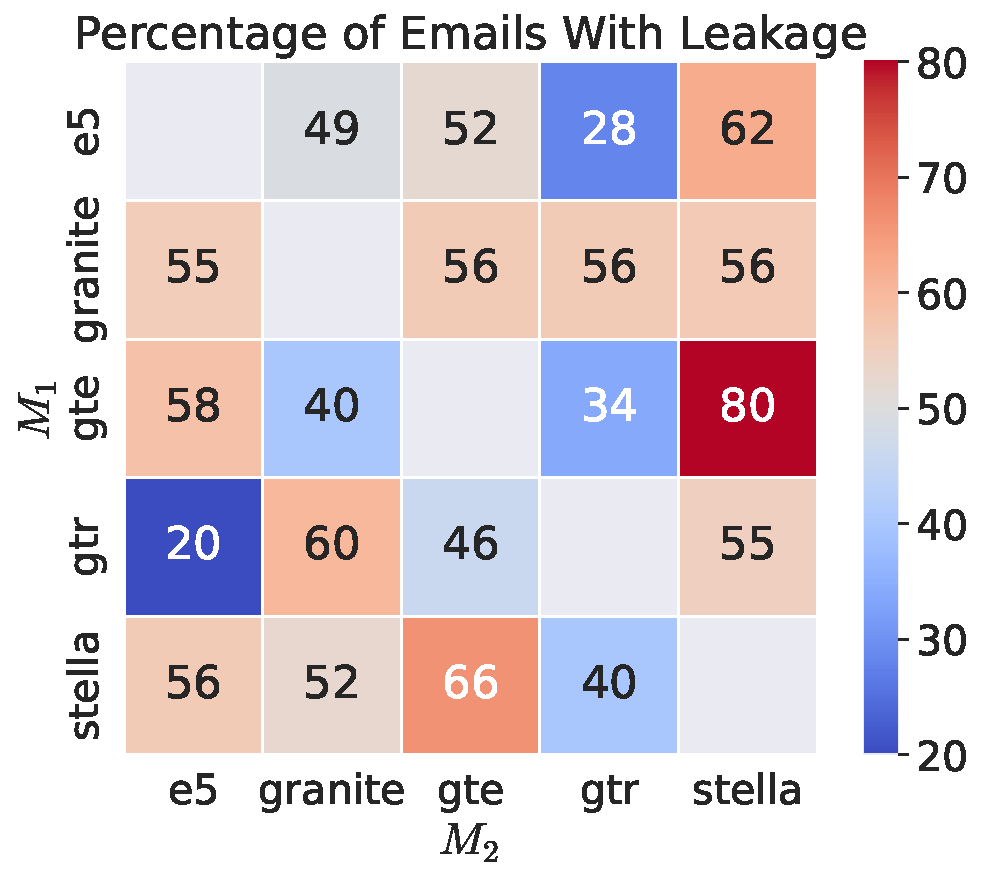
\includegraphics[width=0.5\linewidth]{ims/enron_heatmap.pdf}
%     \caption{Measuring the leakage of information via embedding inversion. \atk{}s trained on NQ and evaluated on a 50-email subset of the Enron Email Corpus. Each cell represents the percentage of reconstructed emails that an LLM judge decided leaked information.}
%     \label{fig:enron_heatmap}
% \end{figure}

\shortpara{Zero-shot inversion.}
Inversion, i.e., reconstruction of text inputs, is more ambitious than attribute inference.  \atk{} translations retain enough semantic information that off-the-shelf, zero-shot inversion methods like~\cite{zhang2025universalzeroshotembeddinginversion}, developed for embeddings computed by standard encoders, extract information for as many as 80\% of documents given \emph{only} their translated embeddings, for some model pairs (\Cref{fig:enron_heatmap}).  These inversions are imperfect and we leave development of specialized inverters for translated embeddings to future work.  Nevertheless, as exemplified in \Cref{fig:inversion_example}, they still extract information such as individual and company names, dates, promotions, financial information, outages, and even lunch orders. In \Cref{sec:prompt}, we show the prompt we use to measure extraction.

\begin{figure}[ht]
  \centering
    \begin{callout}
    \textbf{Ground Truth:} ``Subject: \colorbox{green}{Enron} \colorbox{yellow}{Bashing} on Frontline \verb|\n| Body:..."\\
    \textbf{Generation:} ``Some emails discussing \colorbox{green}{NROn} Employee/s \colorbox{yellow}{Complaint To thePublic}..."\\
    
    \textbf{Ground Truth:} ``Subject: \colorbox{yellow}{Trades for 3/1/02} \verb|\n| Body: \verb|\n| \colorbox{green}{John}, \verb|\n| The following trades..."\\
    \textbf{Generation:} ``... \colorbox{yellow}{future transactions} may await \colorbox{green}{John} G..."\\

    \textbf{Ground Truth:} ``\colorbox{yellow}{The following expense report} is ready for approval..."\\
    \textbf{Generation:} ``\colorbox{yellow}{The upcoming expense statement} from YYYY MM Dec..."    
    \end{callout}
  \caption{Examples of inversions that infer \colorbox{green}{entities} and \colorbox{yellow}{content}.}
  \label{fig:inversion_example}
\end{figure}







% e5 -> gte: 52\%
% \begin{verbatim}
% {
%     "ground_truth": "Subject: \n Body: \n IMPORTANT MESSAGE! PLEASE READ! \n FILENET SYSTEM OUTAGE \n NOVEMBER 30, 2001 \n The FileNET System will be down for offline backups beginning today, November 30th at 5:00pm",
%     "generation": "Today's computers encountered an abrupt stop during communications and affected customer synchronization dates as scheduled backups of critical business information had their timestamp outlastd until after service reactivation",
% },
% \end{verbatim}

% gte -> gtr: 34\%



% Old data:
% \begin{table}[h]
%     \centering
%     \begin{tabular}{llccc|cc|ccc}
%         \toprule
%         \multicolumn{2}{c}{} & \multicolumn{3}{c}{Embedding} & \multicolumn{2}{c}{Text Inversion} & \multicolumn{3}{c}{Extraction (Top-3)} \\
%         \cmidrule(lr){3-5} \cmidrule(lr){6-7} \cmidrule(lr){8-10}
%         $E_1$ & $E_2$ & $\cos(\cdot)$ & Top-1 & Rank & $\cos(\cdot)$ & Token-F1 & $E_1 \to E_2$ & $E_1$ & $E_2$ \\
%         \midrule
%         gte & gtr & 0.70 & 0.80 & 1.78 & 0.58 & 0.10 & 0.01 & 0.99 & 0.97 \\
%         gtr & gte & 0.83 & 0.76 & 2.33 & - & - & 0.01 & 0.97 & 0.99 \\
%         stella & gte & 0.90 & 1.00 & 1.00 & - & - & 0.43 & 0.89 & 0.99 \\
%         gte & stella & 0.86 & 1.00 & 1.00 & - & - & 0.27 & 0.99 & 0.89 \\
%         s-t5 & gtr & 0.85 & 1.00 & 1.00 & 0.67 & 0.14 & 0.83 & 0.92 & 0.97 \\
%         gtr & s-t5 & 0.93 & 1.00 & 1.00 & - & - & 0.67 & 0.97 & 0.92 \\
%         \bottomrule
%     \end{tabular}
%     \caption{Full name extraction! GANs trained on NQ and evaluated on Enron (out-of-distribution)}
%     \label{tab:embedding_comparison}
% \end{table}
